\documentclass[10pt]{article}
\textwidth = 6.5in
\textheight = 9in
\hoffset=-.75in
\voffset=-.8in

\usepackage[pass]{geometry}
%\usepackage[hypertex]{hyperref}
\usepackage{hyperref}
\usepackage{lastpage}
\usepackage{fancyhdr}
\usepackage{sectsty}
\usepackage{amsmath}
%\usepackage{changepage}
\usepackage{scrextend}

\usepackage{graphicx}
\graphicspath{ {./images/} }



\sectionfont{\Large\sf\bfseries}
\subsectionfont{\large\sf\bfseries}

\pagestyle{fancy}
% supress normal headings and footters
\fancyhf{}
% remove the heading rule
\renewcommand{\headrulewidth}{0pt}

\lfoot{{\sf\scriptsize Copyright \copyright\ 2019, 2020, 2021 John Winans.  All Rights Reserved}\\
{\scriptsize\FooterText}}
%\lfoot{\scriptsize\FooterText}

\rfoot{Page \thepage\ of \pageref*{LastPage}}

% Sub-footer that shows the VCS Header in the lfoot defined above
\ifdefined\GitFileName
    \newcommand{\FooterText}{\tt \GitFileName\\
\GitDescription}
\else
    \newcommand{\FooterText}{\emph{--UNKNOWN--}}
\fi


\setlength{\parindent}{0pt}
\setlength{\parskip}{.51em}

% do not number the sections
%\setcounter{secnumdepth}{0}

\begin{document}
%\pagenumbering{gobble}

\title{Boolean Algebra}
\author{John Winans}
%\date{December 2004}
\maketitle
\thispagestyle{fancy}


%%%%%%%%%%%%%%%%%%%%%%%%%%%%%%%%%%%%%%%%%%%%%%%%%%%%%%%%%%%%%%%%%%%
\section{Basic Operations}

We describe Boolean values as either {\em false} or {\em true}.\footnote{
In non-binary systems it might help to consider a more general definition where 
zero is considered {\em false} and anything that is not {\em false} is {\em true}.}

In a system that represents information numerically using only binary digits:

\begin{itemize}
\item 0 = {\em false}
\item 1 = {\em true}
\end{itemize}



The following three basic Boolean operations represent the only operators we 
will use when reducing equations into their simplest form.

%%%%%%%%%%%%%%%%%%%%%%%%%%%%%%%%%%%%%%%%%%%%%%%%%%%%%%%%%%%%%%%%%%%
\subsection{NOT}

A function whose output is the opposite of its input.

\begin{align}
Q &= \overline{A}
\end{align}

\begin{center}
\begin{tabular}{|c|c|}
\hline
A & Q \\
\hline
0 & 1 \\
1 & 0 \\
\hline
\end{tabular}

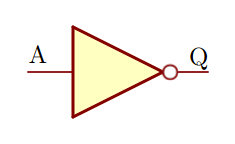
\includegraphics[width=3cm]{not.png}
\end{center}

Depending on the context, any of the following forms might be seen used to 
express the {\bfseries NOT} function applied to the variable $a$:

\begin{itemize}
\item $\neg a$
\item $\overline{a}$
\item $a'$
\item \verb@~a@ (C bitwise operator)
\item \verb@!a@ (C logical operator)
\end{itemize}



%%%%%%%%%%%%%%%%%%%%%%%%%%%%%%%%%%%%%%%%%%%%%%%%%%%%%%%%%%%%%%%%%%%
\subsection{AND}

A function whose output is {\em true} if, and only if, all of its inputs are {\em true}.

\begin{align}
Q &= A \land B
\end{align}

\begin{center}
\begin{tabular}{|cc|c|}
\hline
A & B & Q \\
\hline
0 & 0 & 0 \\
0 & 1 & 0 \\
1 & 0 & 0 \\
1 & 1 & 1 \\
\hline
\end{tabular}

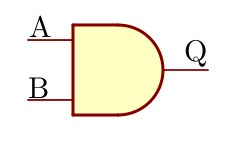
\includegraphics[width=3cm]{and.png}
\end{center}

%\begin{align}
%Q &= A \land B \land C
%\end{align}
%
%\begin{center}
%\begin{tabular}{|ccc|c|}
%\hline
%A & B & C & Q \\
%\hline
%0 & 0 & 0 & 0 \\
%0 & 0 & 1 & 0 \\
%0 & 1 & 0 & 0 \\
%0 & 1 & 1 & 0 \\
%1 & 0 & 0 & 0 \\
%1 & 0 & 1 & 0 \\
%1 & 1 & 0 & 0 \\
%1 & 1 & 1 & 1 \\
%\hline
%\end{tabular}
%\end{center}

Depending on the context, any of the following forms might be seen used to 
express the {\bfseries AND} function applied to the variables $a$ and $b$

\begin{itemize}
\item $a\land b$
\item $a\cdot b$
\item $ab$
\item \verb@a & b@ (C bitwise operator)
\item \verb@a && b@ (C logical operator)
\end{itemize}

%%%%%%%%%%%%%%%%%%%%%%%%%%%%%%%%%%%%%%%%%%%%%%%%%%%%%%%%%%%%%%%%%%%
\subsection{OR}

A function whose output is {\em true} if any one, or both, of its inputs is/are {\em true}.

\begin{align}
Q &= A \lor B
\end{align}

\begin{center}
\begin{tabular}{|cc|c|}
\hline
A & B & Q \\
\hline
0 & 0 & 0 \\
0 & 1 & 1 \\
1 & 0 & 1 \\
1 & 1 & 1 \\
\hline
\end{tabular}

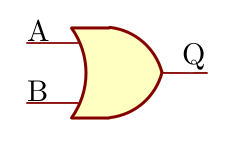
\includegraphics[width=3cm]{or.png}\\
\end{center}

%\begin{align}
%Q &= A \lor B \lor C
%\end{align}
%
%\begin{center}
%\begin{tabular}{|ccc|c|}
%\hline
%A & B & C & Q \\
%\hline
%0 & 0 & 0 & 0 \\
%0 & 0 & 1 & 1 \\
%0 & 1 & 0 & 1 \\
%0 & 1 & 1 & 1 \\
%1 & 0 & 0 & 1 \\
%1 & 0 & 1 & 1 \\
%1 & 1 & 0 & 1 \\
%1 & 1 & 1 & 1 \\
%\hline
%\end{tabular}
%\end{center}

Depending on the context, any of the following forms might be seen used to 
express the {\bfseries OR} function applied to the variables $a$ and $b$

\begin{itemize}
\item $a\lor b$
\item $a+b$
\item \verb@a | b@ (C bitwise operator)
\item \verb@a || b@ (C logical operator)
\end{itemize}

%%%%%%%%%%%%%%%%%%%%%%%%%%%%%%%%%%%%%%%%%%%%%%%%%%%%%%%%%%%%%%%%%%%
\section{Composing New Functions}

We can combine the above three functions to create new ones.

%%%%%%%%%%%%%%%%%%%%%%%%%%%%%%%%%%%%%%%%%%%%%%%%%%%%%%%%%%%%%%%%%%%
\subsection{NAND}

A function whose output is {\em false} if, and only if, all of its inputs are {\em true}.

\begin{align}
Q &= \overline{A \land B}
\end{align}

\begin{center}
\begin{tabular}{|cc|c|}
\hline
A & B & Q \\
\hline
0 & 0 & 1 \\
0 & 1 & 1 \\
1 & 0 & 1 \\
1 & 1 & 0 \\
\hline
\end{tabular}

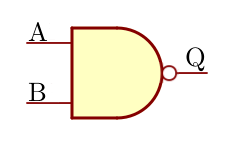
\includegraphics[width=3cm]{nand.png}
\end{center}

%\begin{align}
%Q &= \overline{A \land B \land C}
%\end{align}
%
%\begin{center}
%\begin{tabular}{|ccc|c|}
%\hline
%A & B & C & Q \\
%\hline
%0 & 0 & 0 & 1 \\
%0 & 0 & 1 & 1 \\
%0 & 1 & 0 & 1 \\
%0 & 1 & 1 & 1 \\
%1 & 0 & 0 & 1 \\
%1 & 0 & 1 & 1 \\
%1 & 1 & 0 & 1 \\
%1 & 1 & 1 & 0 \\
%\hline
%\end{tabular}
%\end{center}

Depending on the context, any of the following forms might be seen used to 
express the {\bfseries NAND} function applied to the variables $a$ and $b$

\begin{itemize}
\item $\overline{a\land b}$
\item $\overline{ab}$
\item $\overline{a\cdot b}$
\item \verb@~(a & b)@ (C bitwise operators)
\item \verb@!(a && b)@ (C logical operators)
\end{itemize}

%%%%%%%%%%%%%%%%%%%%%%%%%%%%%%%%%%%%%%%%%%%%%%%%%%%%%%%%%%%%%%%%%%%

\subsection{NOR}

A function whose output is {\em true} if, and only if, all of its inputs are {\em false}.

\begin{align}
Q &= \overline{A \lor B}
\end{align}

\begin{center}
\begin{tabular}{|cc|c|}
\hline
A & B & Q \\
\hline
0 & 0 & 1 \\
0 & 1 & 0 \\
1 & 0 & 0 \\
1 & 1 & 0 \\
\hline
\end{tabular}

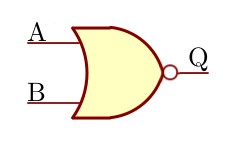
\includegraphics[width=3cm]{nor.png}
\end{center}

Depending on the context, any of the following forms might be seen used to 
express the {\bfseries NOR} function applied to the variables $a$ and $b$

\begin{itemize}
\item $\overline{a\lor b}$
\item $\overline{a+b}$
\item \verb@~(a | b)@ (C bitwise operators)
\item \verb@!(a || b)@ (C logical operators)
\end{itemize}


%%%%%%%%%%%%%%%%%%%%%%%%%%%%%%%%%%%%%%%%%%%%%%%%%%%%%%%%%%%%%%%%%%%
\subsection{XOR (Exclusive OR)}

A function whose output is {\em true} when an odd number of its 
inputs are {\em true}.  We call this {\em odd parity}.  In the special case 
(when there are only two inputs) the {\bfseries XOR} function output is {\em true}
when the two inputs are different and {\em false} when they are the same.

\begin{align}
Q &= A \oplus B \\
  &= \overline{A} \land B \lor A \land \overline{B}
\end{align}

\begin{center}
\begin{tabular}{|cc|c|}
\hline
A & B & Q \\
\hline
0 & 0 & 0 \\
0 & 1 & 1 \\
1 & 0 & 1 \\
1 & 1 & 0 \\
\hline
\end{tabular}

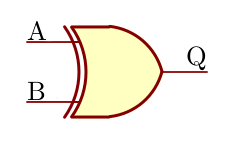
\includegraphics[width=3cm]{xor.png}
\end{center}

Depending on the context, any of the following forms might be seen used to 
express the {\bfseries XOR} function applied to the variables $a$ and $b$

\begin{itemize}
\item $a \oplus b$
\item \verb@a ^ b@ (C bitwise operator)
\end{itemize}

%%%%%%%%%%%%%%%%%%%%%%%%%%%%%%%%%%%%%%%%%%%%%%%%%%%%%%%%%%%%%%%%%%%
\section{Material Implication}

A function with two inputs $a$ and $b$ whose output is {\em true} if either $a$ is 
{\em false} or $a$ is {\em true} when $b$ is {\em true}.

\begin{align}
Q & = A \rightarrow B\\
%  & = \overline{A} \lor A \land B\\
  & = \overline{A} \lor B 
\end{align}

\begin{center}
\begin{tabular}{|cc|c|}
\hline
A & B & Q \\
\hline
0 & 0 & 1 \\
0 & 1 & 1 \\
1 & 0 & 0 \\
1 & 1 & 1 \\
\hline
\end{tabular}
\end{center}

Depending on the context, any of the following forms might be seen used to 
express the {\bfseries IMP} function applied to the variables $a$ and $b$


\begin{itemize}
\item $a \rightarrow b$
\item \verb@a ? b : true@ (C conditional/ternary operator)
\end{itemize}



%%%%%%%%%%%%%%%%%%%%%%%%%%%%%%%%%%%%%%%%%%%%%%%%%%%%%%%%%%%%%%%%%%%
\section{All Possible Functions With Two Inputs}

Consider the following:
\begin{itemize}
\item How many ways can we arrange 2 bits?  (Answer: $2^2 = 4$)
\item How many ways can we arrange 4 bits?  (Answer: $2^4 = 16$)
\end{itemize}

Therefore:

\begin{enumerate}
\item There are exactly four possible ways to arrange two one-bit values.
\item There are exactly sixteen possible ways to arrange four one-bit values. 
\end{enumerate}

Conclusion: There are 16 possible Boolean functions that have two one-bit inputs $a$ and $b$:

\begin{center}
\begin{tabular}{|cc|cccccccccccccccc|}
% \hline  XXX can't see the overlines very well :-/
$a$ & $b$ & 
	0 &
	$a\land b$ &
	$\overline{a\rightarrow b}$ &
	$a$ &
	$\overline{b\rightarrow a}$ &
	$b$ &
	$a\oplus b$ &
	$a\lor b$ &
	$\overline{a\lor b}$ &
	$\overline{a\oplus b}$ &
	$\overline{b}$ &
	$b\rightarrow a$ &
	$\overline{a}$ &
	$a\rightarrow b$ &
	$\overline{a\land b}$ &
	1 \\
\hline
0 & 0 & 0 & 0 & 0 & 0 & 0 & 0 & 0 & 0 & 1 & 1 & 1 & 1 & 1 & 1 & 1 & 1 \\
0 & 1 & 0 & 0 & 0 & 0 & 1 & 1 & 1 & 1 & 0 & 0 & 0 & 0 & 1 & 1 & 1 & 1 \\
1 & 0 & 0 & 0 & 1 & 1 & 0 & 0 & 1 & 1 & 0 & 0 & 1 & 1 & 0 & 0 & 1 & 1 \\
1 & 1 & 0 & 1 & 0 & 1 & 0 & 1 & 0 & 1 & 0 & 1 & 0 & 1 & 0 & 1 & 0 & 1 \\
\hline
  &   & 0 & 1 & 2 & 3 & 4 & 5 & 6 & 7 & 8 & 9 & a & b & c & d & e & f \\
\hline
\end{tabular}
\end{center}



%\begin{verbatim}
%16 possible 2-in 1-out boolean functions
%
%a b  0 a&b ~(a->b) a ~(~a->~b) b a^b a|b ~(a|b) ~(a^b) ~b ~a->~b ~a a->b ~(a&b) 1
%----------------------------------------------------------------------------------
%0 0  0  0     0    0      0    0  0   0     1      1    1    1    1  1      1   1
%0 1  0  0     0    0      1    1  1   1     0      0    0    0    1  1      1   1
%1 0  0  0     1    1      0    0  1   1     0      0    1    1    0  0      1   1
%1 1  0  1     0    1      0    1  0   1     0      1    0    1    0  1      0   1
%----------------------------------------------------------------------------------
%     0  1     2    3      4    5  6   7     8      9    a    b    c  d      e   f
%\end{verbatim}

%%%%%%%%%%%%%%%%%%%%%%%%%%%%%%%%%%%%%%%%%%%%%%%%%%%%%%%%%%%%%%%%%%%
\section{DeMorgan's Morgan's Laws}

\url{https://en.m.wikipedia.org/wiki/De_Morgan's_laws}

%\url{https://www.csus.edu/indiv/p/pangj/class/cpe64/ademo/L1_Demo_Demorgan.pdf}

De Morgan observed the following relationships:

%\begin{align}
%A \land B &= \overline{\overline{A} \lor \overline{B}} \\
%A\lor B &= \overline{\overline{A} \land \overline{B}}
%\end{align}
%
%By taking the {\em NOT} of both sides in the above equations, we get the
%following equivalent equations: 

\begin{align}
\overline{a \land b} &= \overline{a} \lor \overline{b} \\
\overline{a \lor b} &= \overline{a} \land \overline{b}
\end{align}

Proof by truth table:

\begin{center}
\begin{tabular}{|cc|cccccccc|}
%\hline
a & b & 
		$\overline{a}$ &
		$\overline{b}$ &
		$a\land b$ & 
		$\overline{a \land b}$ & 
		$\overline{a}\lor\overline{b}$ &
		$a \lor b$ &
		$\overline{a \lor b}$ &
		$\overline{a} \land \overline{b}$ \\
\hline
0 & 0 & 1 & 1 & 0 & 1 & 1 & 0 & 1 & 1 \\
0 & 1 & 1 & 0 & 0 & 1 & 1 & 1 & 0 & 0 \\
1 & 0 & 0 & 1 & 0 & 1 & 1 & 1 & 0 & 0 \\
1 & 1 & 0 & 0 & 1 & 0 & 0 & 1 & 0 & 0 \\
\hline
\end{tabular}
\end{center}



%%%%%%%%%%%%%%%%%%%%%%%%%%%%%%%%%%%%%%%%%%%%%%%%%%%%%%%%%%%%%%%%%%%%%%%%%%%%%%%%%%%%%%%%%%
\section{Completeness}

{\em Completeness} refers to the fact that the {\em basic operations}
provide a sufficient basis to describe all other possible Boolean
operations.

\url{https://en.wikipedia.org/wiki/Boolean_algebra#Completeness}


A proof showing that NAND is {\em complete} by showing a truth table 
for a NOT, AND and OR function that are constructed only using 
the NAND function.
\footnote{This along with DeMorgan's laws and the above discussion on the
composition of new functions demonstrates that the NAND function alone
can be used to perform all 16 possible Boolean functions.}

\begin{align}
\overline{a} &= \overline{a\land a} \\
a\land b &= \overline{\overline{a\land b}\land\overline{a\land b}}	\\
a\lor b &= \overline{\overline{a\land a}\land\overline{b\land b}}
\end{align}

\begin{center}
\begin{tabular}{|cc|ccccccccc|}
%\hline
a & b & 
		$\overline{a}$ &
		$\overline{a\land a}$ &
		$\overline{b\land b}$ &
		$\overline{a\land a}\land\overline{b\land b}$ &
		$\overline{\overline{a\land a}\land\overline{b\land b}}$ &
		$a\lor b$ &
		$\overline{a\land b}$ &
		$\overline{\overline{a\land b}\land\overline{a\land b}}$ &
		$a\land b$
		\\
\hline
0 & 0 & 1 & 1 & 1 & 1 & 0 & 0 & 1 & 0 & 0 \\
0 & 1 & 1 & 1 & 0 & 0 & 1 & 1 & 1 & 0 & 0 \\
1 & 0 & 0 & 0 & 1 & 0 & 1 & 1 & 1 & 0 & 0 \\
1 & 1 & 0 & 0 & 0 & 0 & 1 & 1 & 0 & 1 & 1 \\
\hline
\end{tabular}
\end{center}


%%%%%%%%%%%%%%%%%%%%%%%%%%%%%%%%%%%%%%%%%%%%%%%%%%%%%%%%%%%%%%%%%%%
\section{Operator Precedence \& Parenthesis}

\begin{itemize}
\item The NOT operator has higher precedence than AND.
\item The AND operator has higher precedence than OR.
\item The OR operator has higher precedence than IMPLICATION.
\end{itemize}

{\em Note that XOR is a function of one or more of these operators.  
Therefore its precedence is a matter of its implementation.  
Languages like C that include an explicit XOR operator put its 
precedence between that of the AND and OR operators.}

Parenthesis can be used to manage the order of operations when the
precedence rules would otherwise cause an undesirable result:

\begin{align}
a \lor b \land c & = a \lor ( b \land c ) \\
& \neq ( a \lor b ) \land c
\end{align}


\section{Laws of Boolean Algebra}

Summarized from \url{https://en.wikipedia.org/wiki/Boolean_algebra}.

\begin{align}
a \land ( b \land c ) & = ( a \land b ) \land c	&& \text{Associativity of } \land \\
a \lor ( b \lor c ) & = ( a \lor b ) \lor c		&& \text{Associativity of } \lor \\
a \land b & = b \land a							&&  \text{Commutativity of } \land \\
a \lor b & = b \lor a							&&  \text{Commutativity of } \lor \\
a \land ( b \lor c) & = (a \land b) \lor (a \land c) && \text{Distributivity of } \land \text{ over } \lor \\
a \lor ( b \land c) & = (a \lor b) \land (a \lor c) && \text{Distributivity of } \lor \text{ over } \land \\
a \land 1 & = a									&& \text{Identity for } \land \\
a \lor 0 & = a									&& \text{Identity for } \lor \\
a \land 0 & = 0									&& \text{Annihilator for } \land \\
a \lor 1 & = 1									&& \text{Annihilator for } \lor \\
a \land a & = a									&& \text{Idempotence } \land \\
a \lor a & = a									&& \text{Idempotence } \lor \\
a \land ( a \lor b ) & = a						&& \text{Absorption 1} \\
a \lor ( a \land b ) & = a						&& \text{Absorption 2} \\
a \land \overline{a} & = 0						&& \text{Complementation of $\land$} \\
a \lor \overline{a} & = 1						&& \text{Complementation of $\lor$} \\
\overline{\overline{a}} & = a					&& \text{Double negation} \\
\overline{a}\land\overline{b} & = \overline{a\lor b}	&& \text{DeMorgan's 1} \\
\overline{a}\lor\overline{b} & = \overline{a\land b}	&& \text{DeMorgan's 2}
\end{align}

\subsection{An Exercise}
You should be able to show that each of the following equations are true
by applying the above Boolean laws and by showing the truth tables for
each case.


\begin{align}
a \land b &= \overline{\overline{a} \lor \overline{b}}		\\
a \lor b &= \overline{\overline{a} \land \overline{b}}		\\
a \lor \overline{a} \land b &= a \lor b						\\
\overline{a} \lor a \land b &= \overline{a} \lor b			\label{function:imp}\\
(a \lor b) \land (c \lor d) & = a \land c \lor a \land d \lor b \land c \lor b \land d
\end{align}

For example, a proof of Equation~\ref*{function:imp}:

\begin{align}
f &= \overline{a} \lor a \land b						&& \text{Given} \\
&= \overline{a} \lor ( a \land b )						&& \text{Show operator precedence} \\
&= (\overline{a} \lor a) \land (\overline{a} \lor b)	&& \text{Distributivity of $\lor$ over $\land$} \\
&= (a \lor \overline{a}) \land (\overline{a} \lor b)	&& \text{Commutativity of $\lor$} \\
&= 1 \land (\overline{a} \lor b)						&& \text{Complementation of $\lor$} \\
&= (\overline{a} \lor b) \land 1						&& \text{Commutativity of $\land$} \\
&= \overline{a} \lor b									&& \text{Identity for $\land$}
\end{align}



%%%%%%%%%%%%%%%%%%%%%%%%%%%%%%%%%%%%%%%%%%%%%%%%%%%%%%%%%%%%%%%%%%%%%%%%%%
\section{Minterm (lower-case m) (SOP form)}

See also: \url{https://en.wikipedia.org/wiki/Canonical_normal_form}

Any Boolean function can be expressed in SOP form.
\footnote{See: Peter J. Pahl, Rudolf Damrath, ``Mathematical Foundations of Computational Engineering: A Handbook,'' 2001, Springer, page 15. \url{https://tinyurl.com/ujv8q7l} }

In a minterm, each variable may appear only once as $a$ or $\overline{a}$.
For a three-input function, there are $2^3 = 8$  minterms:

\begin{align}
m0 & = \overline{a} \land \overline{b} \land \overline{c} \\
m1 & = \overline{a} \land \overline{b} \land c \\
m2 & = \overline{a} \land b \land \overline{c} \\
m3 & = \overline{a} \land b \land c \\
m4 & = a \land \overline{b} \land \overline{c} \\
m5 & = a \land \overline{b} \land c \\
m6 & = a \land b \land \overline{c} \\
m7 & = a \land b \land c
\end{align}

Note that the appearance of the NOT-bars match the pattern of zeros when counting
from zero to seven in binary.

Use of minterms in an equation allows a shorter notation as shown below:

\begin{align}
f & = m1 \lor m2 \lor m4 \lor m7 \\
&= (\overline{a} \land \overline{b} \land c) \lor 
	(\overline{a} \land b \land \overline{c}) \lor 
	(a \land \overline{b} \land \overline{c}) \lor 
	(a \land b \land c) 	\label{pos:example}
\end{align}

{\em Parenthesis added for readability.}

The long form shown in equation~\ref{pos:example} suggests a rationale for why it is called SOP (Sum Of Products.)

\begin{center}
\begin{tabular}{|c|ccc|cccc|c|}
%\hline
     & $a$ & $b$ & $c$ & 
		$(\overline{a} \land \overline{b} \land c)$ &
		$(\overline{a} \land b \land \overline{c})$ &
		$(a \land \overline{b} \land \overline{c})$ &
		$(a \land b \land c)$ &
		$f$ \\
\hline
$m0$ & 0 & 0 & 0 &  0 & 0 & 0 & 0 & 0\\
$m1$ & 0 & 0 & 1 &  1 & 0 & 0 & 0 & 1\\
$m2$ & 0 & 1 & 0 &  0 & 1 & 0 & 0 & 1\\
$m3$ & 0 & 1 & 1 &  0 & 0 & 0 & 0 & 0\\
$m4$ & 1 & 0 & 0 &  0 & 0 & 1 & 0 & 1\\
$m5$ & 1 & 0 & 1 &  0 & 0 & 0 & 0 & 0\\
$m6$ & 1 & 1 & 0 &  0 & 0 & 0 & 0 & 0\\
$m7$ & 1 & 1 & 1 &  0 & 0 & 0 & 1 & 1\\
\hline
\end{tabular}
\end{center}

As can be seen in the truth table, the ``mechanics'' driving the SOP equation is based
on identifying those specific function input patterns where the output is {\em true}.
By using an OR gate to drive the output, it will set its output {\em true} any time one 
of the recognized input terms is {\em true}.

%%%%%%%%%%%%%%%%%%%%%%%%%%%%%%%%%%%%%%%%%%%%%%%%%%%%%%%%%%%%%%%%%%%%%%%%%%
\section{Maxterm (upper-case M) (POS form)}

Same idea as the minterm, but inverted and use the $\lor$ instead of the $\land$ function:

Any Boolean function can be expressed in POS form.


\begin{align}
M0 & = a \lor b \lor c \\
M1 & = a \lor b \lor \overline{c} \\
M2 & = a \lor \overline{b} \lor c \\
M3 & = a \lor \overline{b} \lor \overline{c} \\
M4 & = \overline{a} \lor b \lor c \\
M5 & = \overline{a} \lor b \lor \overline{c} \\
M6 & = \overline{a} \lor \overline{b} \lor c \\
M7 & = \overline{a} \lor \overline{b} \lor \overline{c}
\end{align}

Note that the appearance of the NOT-bars match the pattern of ones when counting
from zero to seven in binary.

\begin{align}
f &= M0 \land M1 \land M2 \land M4 \\
&= (a \lor b \lor c) \land 
	(a \lor b \lor \overline{c}) \land
	(a \lor \overline{b} \lor c) \land
	(\overline{a} \lor b \lor c) \label{sop:example}
\end{align}

The long form shown in equation~\ref{sop:example} is often called a POS (Product Of Sums.)

\begin{center}
\begin{tabular}{|c|ccc|cccc|c|}
%\hline
     & $a$ & $b$ & $c$ & 
		$(a \lor b \lor c)$ &
		$(a \lor b \lor \overline{c})$ &
		$(a \lor \overline{b} \lor c)$ &
		$(\overline{a} \lor b \lor c)$ &
		$f$ \\
\hline
$M0$ & 0 & 0 & 0 &  0 & 1 & 1 & 1 & 0\\
$M1$ & 0 & 0 & 1 &  1 & 0 & 1 & 1 & 0\\
$M2$ & 0 & 1 & 0 &  1 & 1 & 0 & 1 & 0\\
$M3$ & 0 & 1 & 1 &  1 & 1 & 1 & 1 & 1\\
$M4$ & 1 & 0 & 0 &  1 & 1 & 1 & 0 & 0\\
$M5$ & 1 & 0 & 1 &  1 & 1 & 1 & 1 & 1\\
$M6$ & 1 & 1 & 0 &  1 & 1 & 1 & 1 & 1\\
$M7$ & 1 & 1 & 1 &  1 & 1 & 1 & 1 & 1\\
\hline
\end{tabular}
\end{center}

As can be seen in the truth table, the ``mechanics'' driving the POS equation is based
on identifying those specific function input patterns where the output is {\em false}.
By using an AND to drive the output, it will set its output {\em false} any time one 
of the recognized input terms is {\em false}.


%%%%%%%%%%%%%%%%%%%%%%%%%%%%%%%%%%%%%%%%%%%%%%%%%%%%%%%%%%%%%%%%%%%%%%%%%%
\subsection{Relationship Between Minterms and Maxterms}

The complement of a maxterm, such as $\overline{M5}$, is the respective minterm $m5$.

This can be verified with DeMorgan's as in:

\begin{align}
M5 & = \overline{a} \lor b \lor \overline{c}	&& \text{Given}		\\
m5 & = a \land \overline{b} \land c				&& \text{Given}		\\
\overline{M5} & = \overline{\overline{a} \lor b \lor \overline{c}}	&& \text{Complement both sides} \\
\overline{M5} & = \overline{\overline{a}} \land \overline{b} \land \overline{\overline{c}}	&& \text{DeMorgan 1} \\
\overline{M5} & = a \land \overline{b} \land c				&& \text{Double negation} \\
% \overline{M5} & = a \land \overline{b} \land c				&& \text{DeMorgan's 1} \\
\overline{M5} & = m5
\end{align}

Note that DeMorgan's also works with more than two inputs.

It turns out that converting a minterm to a maxterm works the same way. 
For example:

\begin{align}
M5 & = \overline{a} \lor b \lor \overline{c}	&& \text{Given}		\\
m5 &= a \land \overline{b} \land c		&& \text{Given}		\\
\overline{m5} &= \overline{a \land \overline{b} \land c}	&& \text{Complement both sides} \\
\overline{m5} &= \overline{a} \lor \overline{\overline{b}} \lor \overline{c}	&& \text{DeMorgan 2} \\
\overline{m5} &= \overline{a} \lor b \lor \overline{c}			&& \text{Double negation} \\
% &= \overline{a} \lor b \lor \overline{c}			&& \text{DeMorgan's 2} \\
\overline{m5} &= M5
\end{align}

%%%%%%%%%%%%%%%%%%%%%%%%%%%%%%%%%%%%%%%%%%%%%%%%%%%%%%%%%%%%%%%%%%%%%%%%%%
\subsection{When to Apply the POS or SOP Form}

If SOP and POS can be easily converted back and forth, it begs the question
``Why concern ourselves with both forms?''

The answer lies in which of the two forms is easier to apply to a given
situation.  For example, the following truth table is best expressed in SOP 
form simply because there are fewer cases when the output is {\em true}. 

\begin{center}
\begin{tabular}{|ccc|c|}
%\hline
$a$ & $b$ & $c$ & $f$ \\
\hline
 0 & 0 & 0 &   0\\
 0 & 0 & 1 &   0\\
 0 & 1 & 0 &   0\\
 0 & 1 & 1 &   1\\
 1 & 0 & 0 &   0\\
 1 & 0 & 1 &   1\\
 1 & 1 & 0 &   0\\
 1 & 1 & 1 &   1\\
\hline
\end{tabular}
\end{center}

Therefore there are fewer terms expressed in the SOP form describing it:

\begin{align}
f & = m3 \lor m5 \lor m7 \\
&= (\overline{a} \land b \land c) \lor
	(a \land \overline{b} \land c) \lor
	(a \land b \land c)						\label{eqn:sop:example}
\end{align}

%m0 & = \overline{a} \land \overline{b} \land \overline{c} \\
%m1 & = \overline{a} \land \overline{b} \land c \\
%m2 & = \overline{a} \land b \land \overline{c} \\
%m3 & = \overline{a} \land b \land c \\
%m4 & = a \land \overline{b} \land \overline{c} \\
%m5 & = a \land \overline{b} \land c \\
%m6 & = a \land b \land \overline{c} \\
%m7 & = a \land b \land c

\ldots{}than there are in the POS form:

\begin{align}
f &= M0 \land M1 \land M2 \land M4 \land M6 \\
&= (a \lor b \lor c) \land
	(a \lor b \lor \overline{c}) \land
	(a \lor \overline{b} \lor c) \land
	(\overline{a} \lor b \lor c) \land
	(\overline{a} \lor \overline{b} \lor c)
\end{align}


%M0 & = a \lor b \lor c \\
%M1 & = a \lor b \lor \overline{c} \\
%M2 & = a \lor \overline{b} \lor c \\
%M3 & = a \lor \overline{b} \lor \overline{c} \\
%M4 & = \overline{a} \lor b \lor c \\
%M5 & = \overline{a} \lor b \lor \overline{c} \\
%M6 & = \overline{a} \lor \overline{b} \lor c \\
%M7 & = \overline{a} \lor \overline{b} \lor \overline{c}

The shorter function may be more desirable to work with.

%%%%%%%%%%%%%%%%%%%%%%%%%%%%%%%%%%%%%%%%%%%%%%%%%%%%%%%%%%%%%%%%%%%%%%%%%%
\section{Simplification of SOP and POS Forms}

While it is easy to express any Boolean function in SOP or POS form, it is 
desirable to be able to then reduce them to their simplest form.

To accomplish this, we apply the Boolean laws until the function becomes irreducible and
has the fewest number of operators.

As an example we demonstrate a reduction of the following truth table 
using both the SOP and POS functions:

\begin{center}
\begin{tabular}{|c|ccc|c|}
%\hline
	& $a$ & $b$ & $c$ & $f$ \\
\hline
$0$ & 0 & 0 & 0 &   0\\
$1$ & 0 & 0 & 1 &   0\\
$2$ & 0 & 1 & 0 &   1\\
$3$ & 0 & 1 & 1 &   0\\
$4$ & 1 & 0 & 0 &   1\\
$5$ & 1 & 0 & 1 &   1\\
$6$ & 1 & 1 & 0 &   1\\
$7$ & 1 & 1 & 1 &   1\\
\hline
\end{tabular}
\end{center}


\begin{align}
\text{SOP:}\\
f &= m2 \lor m4 \lor m5 \lor m6 \lor m7 			&& \text{Given} \\
&= ( \overline{a} \land b \land \overline{c} ) \lor 
	( a \land \overline{b} \land \overline{c} ) \lor
	( a \land \overline{b} \land c ) \lor
	( a \land b \land \overline{c} ) \lor
	( a \land b \land c ) 							&& \text{Expand the terms} \\
&= ( \overline{a} \land b \land \overline{c} ) \lor
	( a \land \overline{b} \land (\overline{c} \lor c) ) \lor
	( a \land b \land (\overline{c} \lor c) )		&& \text{Distributive of $\land$ over $\lor$} \\
&= ( \overline{a} \land b \land \overline{c} ) \lor
	( a \land \overline{b} \land 1 ) \lor
	( a \land b \land 1 )							&& \text{Complementation of $\lor$} \\
&= ( \overline{a} \land b \land \overline{c} ) \lor
	( a \land \overline{b} ) \lor
	( a \land b )									&& \text{Identity for $\land$} \\
&= ( \overline{a} \land b \land \overline{c} ) \lor
	( a \land (\overline{b} \lor b) )				&& \text{Distributive of $\land$ over $\lor$} \\
&= ( \overline{a} \land b \land \overline{c} ) \lor
	( a \land 1 )									&& \text{Complementation of $\lor$} \\
&= ( \overline{a} \land b \land \overline{c} ) \lor
	a												&& \text{Identity for $\land$} \\
&= a \lor
	( \overline{a} \land b \land \overline{c} ) 	&& \text{Commutativity of $\lor$} \\
&= a \lor
	( \overline{a} \land ( b \land \overline{c} )) 	&& \text{Associativity of $\land$} \\
&= (a \lor \overline{a}) \land
	(a \lor (b \land \overline{c}) )				&& \text{Distributivity of $\lor$ over $\land$}\\
&= 1 \land (a \lor (b \land \overline{c}) )			&& \text{Complementation of $\lor$} \\
&= a \lor (b \land \overline{c}) 					&& \text{Identity for $\land$} \\
%\end{align}
%
%
%\begin{align}
\text{POS:}\\
f &= M0 \land M1 \land M3 							&& \text{Given} \\
&= (a \lor b \lor c) \land							
	(a \lor b \lor \overline{c}) \land
	(a \lor \overline{b} \lor \overline{c})			&& \text{Expand the terms} \\
&= ((a \lor b) \lor
	(c \land \overline{c})) \land
	(a \lor \overline{b} \lor \overline{c})			&& \text{Distributivity of $\lor$ over $\land$}\\
&= ((a \lor b) \lor
	0) \land
	(a \lor \overline{b} \lor \overline{c})			&& \text{Complementation of $\land$}\\
&= (a \lor b) \land
	(a \lor \overline{b} \lor \overline{c})			&& \text{Identity for $\lor$}\\
&= a \lor (b \land (\overline{b} \lor \overline{c}))	&& \text{Distributivity of $\lor$ over $\land$}\\
&= a \lor ((b \land \overline{b}) \lor 
	(b \land \overline{c}))							&& \text{Distributivity of $\land$ over $\lor$}\\
&= a \lor (0 \lor 
	(b \land \overline{c}))							&& \text{Complementation of $\land$}\\
&= a \lor
	(b \land \overline{c})							&& \text{Identity for $\lor$}\\
\end{align}

Ultimately, we see that both methods arrived at the same conclusion!

	
\end{document}
